


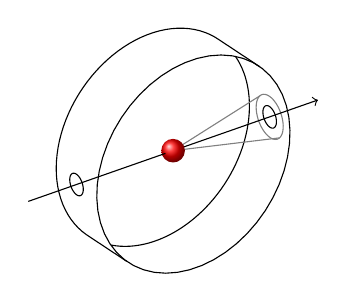
\begin{tikzpicture}
%\useasboundingbox (0,0) rectangle (5,5);
%\draw (2,2) rectangle ++(5,5);


 \begin{axis}[ width=20cm,
   axis lines=none,
    xmin=-2.5,
    xmax=2.5,
    ymin=-2.5,
    ymax=2.5,
    zmin=-2.5,
    zmax=2.5,
    xtick=\empty,
    ytick=\empty,
    ztick=\empty,
    axis equal , rotate around z=60 ,rotate around x=-2 ,
    font=\footnotesize]

%	\addplot3+[ black,
%	no markers,	samples=51, 	samples y=0,	domain=-pi:pi,	variable=\v]
%	(	 {cos(\v r)},{0.3},	 {sin(\v r)}	);   
	
	\addplot3+[ black,
	no markers,	samples=51, 	samples y=0,	domain=45:225,	variable=\v]
	(	 {cos(\v )},{+0.3},	 {sin(\v )}	);   
	
	\addplot3+[ black,
	no markers,	samples=51, 	samples y=0,	domain=243:390,	variable=\v]
	(	 {cos(\v )},{+0.3},	 {sin(\v )}	);   
	
\addplot3+[ black,
	no markers,	samples=51, 	samples y=0,	domain=-pi:pi,	variable=\v]
	(	 {cos(\v r)},{-0.3},	 {sin(\v r)}	);   
	
		\addplot3+[ black,
	no markers,	samples=2, 	samples y=0,	domain=-0.3:0.3,	variable=\v]
	(	 {cos(-135)},{\v},	 {sin( -135)}	);   
			\addplot3+[ black,
	no markers,	samples=2, 	samples y=0,	domain=-0.3:0.3,	variable=\v]
	(	 {cos(45)},{\v},	 {sin( 45)}	);   

	
		\addplot3[ black,
	no markers,	samples=51, 	samples y=0,	domain=-pi:pi,	variable=\v]
	(	{-1}, {0.1 * cos(\v r)},	 {0.1 * sin(\v r)}	);   
	
		\addplot3[ black,
	no markers,	samples=51, 	samples y=0,	domain=-pi:pi,	variable=\v]
	(	{1}, {0.1 * cos(\v r)},	 {0.1 * sin(\v r)}	);   
	
		\addplot3[ gray,
	no markers,	samples=51, 	samples y=0,	domain=-pi:pi,	variable=\v]
	(	{1}, {0.2 * cos(\v r)},	 {0.2 * sin(\v r)}	);   
	
	
  \draw[->](0,0,0) -- (1.5,0,0);
    \draw[gray](0,0,0) -- (1,{0.2 * cos(45)},{0.2 * sin(45)});
    \draw[gray](0,0,0) -- (1,{-0.2 * cos(45)},{-0.2 * sin(45)});

  \shade [ball color=red](0,0,0) circle (1.5mm);

  \draw[-](-1.5,0,0) -- (-0.08,0,0);

  \end{axis}



  
  \end{tikzpicture}




